 \documentclass[oneside,a4paper,12pt]{book}
%\pagestyle{headings}
\frontmatter

%=============================================================================

\usepackage{amsthm}
\usepackage{xspace}
\usepackage{float}
\usepackage{ifthen}
\usepackage{amsbsy}
\usepackage{amssymb}
\usepackage{balance}
\usepackage{booktabs}
\usepackage{graphicx}
\usepackage{rotating}
\usepackage{multirow}
\usepackage{needspace}
\usepackage{microtype}
\usepackage{bold-extra}
\usepackage{geometry}
\usepackage{varioref}
\usepackage{xcolor}
\usepackage{textcomp}
\usepackage{listings}
\usepackage[normalem]{ulem} %emphasize still italic
\usepackage{ucs}

% \usepackage[utf8]{inputenc}
% \usepackage[htt]{hyphenat}
\usepackage{times}
\usepackage{url}
\usepackage{alltt}
\usepackage{amsmath}
\usepackage{xfrac}
\usepackage{subfigure}
\usepackage{appendix}
\usepackage{stmaryrd}   % for the \shortuparrow
\usepackage[utopia]{quotchap}

\usepackage{setspace}
\usepackage[numbers, sort&compress]{natbib}
\usepackage{mdwlist}        % support for better spaced lists
% allows for temporary adjustment of side margins
\usepackage{chngpage}
\usepackage[normalem]{ulem} 

% lina entered
\usepackage{indentfirst}
\usepackage[parfill]{parskip}
\usepackage[bottom]{footmisc}

\usepackage[T1]{fontenc}
\usepackage{caption}
\usepackage{booktabs}
\usepackage{siunitx}


\setlength{\parindent}{1.5em}

% constants

\newcounter{qcounter}

% commands
\newcommand{\n}{$\cdot$}
\newcommand{\y}{\checkmark}
\newcommand{\subscript}[1]{$_{\textrm{\footnotesize{#1}}}$}
\newcommand{\superscript}[1]{$^{\textrm{\footnotesize{#1}}}$}
\newcommand{\vertical}[1]{\raisebox{-4em}{\begin{sideways}{#1}\end{sideways}}}
\newcommand\tab[1][1cm]{\hspace*{#1}}

\usepackage{boxedminipage}

\newboolean{showedits}
\setboolean{showedits}{true} % toggle to show or hide edits
\ifthenelse{\boolean{showedits}}
{
       \newcommand{\ugh}[1]{\textcolor{red}{\uwave{#1}}} % please rephrase
       \newcommand{\ins}[1]{\textcolor{blue}{\uline{#1}}} % please insert
       \newcommand{\del}[1]{\textcolor{red}{\sout{#1}}} % please delete
       \newcommand{\chg}[2]{\textcolor{red}{\sout{#1}}{\ra}\textcolor{blue}{\uline{#2}}} % please change
}{
       \newcommand{\ugh}[1]{#1} % please rephrase
       \newcommand{\ins}[1]{#1} % please insert
       \newcommand{\del}[1]{} % please delete
       \newcommand{\chg}[2]{#2}
}


% ============================================================================
% Put edit comments in a really ugly standout display

\usepackage{xcolor}
\usepackage[normalem]{ulem}
\newcommand{\ra}{$\rightarrow$}
\usepackage{amssymb}

% comments \nb{label}{color}{text}
\newboolean{showcomments}
\setboolean{showcomments}{true}
%\setboolean{showcomments}{false}
\ifthenelse{\boolean{showcomments}}
{\newcommand{\nb}[3]{
  {\colorbox{#2}{\bfseries\sffamily\scriptsize\textcolor{white}{#1}}}
  {\textcolor{#2}{\sf\small$\blacktriangleright$\textit{#3}$\blacktriangleleft$}}}
    \newcommand{\version}{\emph{\scriptsize$-$Id$-$}}
%	 \newcommand{\ugh}[1]{\textcolor{red}{\uwave{#1}}} % please rephrase
%	 \newcommand{\ins}[1]{\textcolor{blue}{\uline{#1}}} % please insert
%	 \newcommand{\del}[1]{\textcolor{red}{\sout{#1}}} % please delete
%	 \newcommand{\chg}[2]{\textcolor{red}{\sout{#1}}{\ra}\textcolor{blue}{\uline{#2}}} % please change
	 \newcommand{\chk}[1]{\textcolor{ForestGreen}{#1}} % changed, please check
	}
{\newcommand{\nb}[3]{}
  \newcommand{\version}{}
  \newcommand{\chk}[1]{} % changed, please check
  }
\newcommand\nm[1]{\nb{NM}{violet}{#1}} % add more author macros here
\newcommand\lt[1]{\nb{LT}{orange}{#1}}


% ============================================================================
% Make quotes be italic
\renewenvironment{quote}
    {\list{}{\rightmargin\leftmargin}%
     \item\relax\begin{it}}
    {\end{it}\endlist}

\newcommand{\ttimes}{\ensuremath{\times}}

%=============================================================================

\newcommand{\needlines}[1]{\Needspace{#1\baselineskip}}

% source code
\usepackage{xcolor}
\usepackage{textcomp}
\usepackage{listings}
\definecolor{javared}{rgb}{0.6,0,0} % for strings
\definecolor{javagreen}{rgb}{0.25,0.5,0.35} % comments
\definecolor{javapurple}{rgb}{0.5,0,0.35} % keywords
\definecolor{javadocblue}{rgb}{0.25,0.35,0.75} % javadoc

\renewcommand{\lstlistingname}{Code}% Listing -> Algorithm
\renewcommand{\lstlistlistingname}{List of \lstlistingname s}% List of Listings -> List of Algorithms

\lstnewenvironment{Java}[1][]
{\lstset{
	language=Java,
	basicstyle=\footnotesize\ttfamily,
	keywordstyle=\color{javapurple}\bfseries,
	stringstyle=\color{javared},
	commentstyle=\color{javagreen},
	morecomment=[s][\color{javadocblue}]{/**}{*/},
	numbers=left,
	numberstyle=\tiny\color{black},
	stepnumber=1,
	numbersep=10pt,
	tabsize=4,
	showspaces=false,
	showstringspaces=false,
	breaklines=true,
	captionpos=b,
	xleftmargin=2em,
	framexleftmargin=1.5em,
	frame=single,
	#1
}}
{}


\lstnewenvironment{JVMIS}[1][]
{\lstset{
	language=JVMIS,
	basicstyle=\footnotesize\ttfamily,
	keywordstyle=\color{javagreen}\bfseries,
	stringstyle=\color{javared},
	commentstyle=\color{javagreen},
	morecomment=[s][\color{javadocblue}]{/**}{*/},
	numbers=none,
	numberstyle=\tiny\color{black},
	stepnumber=1,
	numbersep=10pt,
	tabsize=4,
	showspaces=false,
	showstringspaces=false
	breaklines=true,
	captionpos=b,
	xleftmargin=2em,
	framexleftmargin=1.5em,
	frame=single,
	#1
}}
{}


\definecolor{codegray}{gray}{0.9}
\newcommand{\code}[1]{
	\colorbox{codegray}
	{\texttt{#1}}
}

%----------------------------------------------------------------------------
% references
\newcommand{\tabref}[1]{\hyperref[{tab:#1}]{Table~\ref*{tab:#1}}}
\newcommand{\figref}[1]{\hyperref[{fig:#1}]{Figure~\ref*{fig:#1}}}
\newcommand{\secref}[1]{\hyperref[{sec:#1}]{Section~\ref*{sec:#1}}}
\newcommand{\subsecref}[1]{\hyperref[{subsec:#1}]{Subsection~\ref*{subsec:#1}}}
\newcommand{\lstref}[1]{\hyperref[{lst:#1}]{Listing~\ref*{lst:#1}}}
\newcommand{\charef}[1]{\hyperref[{ch:#1}]{Chapter~\ref*{ch:#1}}}
\newcommand{\coderef}[1]{\hyperref[{code:#1}]{Code~\ref*{code:#1}}}
\newcommand{\bytecoderef}[1]{\hyperref[{bytecode:#1}]{Bytecode~\ref*{bytecode:#1}}}
\newcommand{\algref}[1]{\hyperref[{alg:#1}]{Algorithm~\ref*{alg:#1}}}
\newcommand{\boxref}[1]{\hyperref[{box:#1}]{Box~\ref*{box:#1}}}

%----------------------------------------------------------------------------

% abbreviations
\tracingcolors 4
\setcounter{tocdepth}{3}
\setcounter{secnumdepth}{3}
\newcommand{\ie}{\emph{i.e.,}\xspace}
\newcommand{\eg}{\emph{e.g.,}\xspace}
\newcommand{\etc}{\emph{etc.}\xspace}
\newcommand{\etal}{\emph{et al.}\xspace}


\newcommand{\newevenside}{
	\ifthenelse{\isodd{\thepage}}{\newpage}{
	\newpage
        \phantom{placeholder} % doesn't appear on page
	\thispagestyle{empty} % if want no header/footer
	\newpage
	}
}

\def\stretchfactor{1}
\newcommand{\mychapter}[1]{\setstretch{1}
    \chapter{#1}\setstretch{\stretchfactor}}

%----------------------------------------------------------------------------
\newcommand{\lessSpace}{\vspace{-1em}}
\DeclareGraphicsExtensions{.pdf,.png}
\graphicspath{{images/}}
\newcommand{\fig}[4]{
	\begin{figure}[#1]
		\centering
		\includegraphics[width=#2\textwidth]{#3}
		\lessSpace
		\caption{\label{fig:#3}#4}
	\end{figure}}

% ===========================================================================

%:CONFIGURE THIS

\newcommand{\thesistitle}{Where does this null come from ?}
\newcommand{\thesisauthor}{Lina Tran}
\newcommand{\thesisauthorOrigin}{Biel/Bienne BE, Switzerland}
\newcommand{\thesisleiter}{Prof.\ Dr.\ Oscar Nierstrasz}
\newcommand{\thesisasst}{	\begin{center}
														Research assistant Nevena Milojkovi\'{c}\\
														Research assistant Boris Spasojevi\'{c}
													\end{center}}
\newcommand{\thesisurl}{http://scg.unibe.ch/}
\newcommand{\thesissubtitle}{An Approach to show the exact location where a value was referenced to null}
\newcommand{\thesisdate}{31. July 2016}

% ===========================================================================

\usepackage[ colorlinks=true, urlcolor=black, linkcolor=black,
			citecolor=black, bookmarksnumbered=true, bookmarks=true,
			plainpages=false,
			pdftitle={\thesistitle}, pdfauthor={\thesisauthor},
			pdfsubject={\thesissubtitle}, pdfpagelabels]{hyperref}

\newcommand{\hrref}[2]{\hyperref}
% ===========================================================================
% ===========================================================================


% D O C U M E N T
% % % % % % % % % % % % % % % % % % % % % % % % % % % % % % % % % %
\begin{document}

% T I T L E
% % % % % % % % % % % % % % % % % % % % % % % % % % % % % % % % % %
\begin{titlepage}  
  \begin{center}  
  
  \begin{figure}[t]  
  \vspace*{-2cm}        % to move header logo at the top 
  \center{
\includegraphics[scale=0.5]{logos/UNI_Bern.png}}
  \vspace{1in}     
  \end{figure}

    \thispagestyle{empty}
    
    {\bfseries\Huge \thesistitle \par
    \Large \vspace{0.1in} \thesissubtitle \par}

    \vspace{0.3in} 
    \LARGE{\textbf{Bachelor Thesis} \\}
    \vspace{0.4in}

    {\Large \thesisauthor \par from \par \thesisauthorOrigin}
    
    \vspace{0.3in}
    {\Large Faculty of Science \\
            University of Bern \par}
    \vspace{0.3in}
    {\Large \thesisdate \par}
    \vspace{0.3in}
    %Leiter der Arbeit: \par
   {\Large \thesisleiter} \par
      {\Large \thesisasst} \par
   \vspace{0.1in}
    {\Large Software Composition Group \par Institute for Computer Science \par University of Bern, Switzerland \par}
  

  %\vspace{0.5in}
 
 

  \end{center}

\end{titlepage}


% A B S T R A C T
% % % % % % % % % % % % % % % % % % % % % % % % % % % % % % % % % %
\chapter*{\centering Abstract}
\begin{quotation}
\noindent 
A previous study found out that NullPointerExceptions are very serious in Java projects. When a NullPointerExceptions occurs the developer is provided only with a stack trace to where the exception happened. This only gives insight into the effect of the fault but not into its cause. So we have to ask the question when and why this reference was set to null.

The aim of the project is to be able to provide the user with an additional stack trace of where the value was actually set to null, next to the normal stack trace of an exception. We attempt to achieve this goal by instrumenting java source code ideally with a minimal overhead. 

By tracking the null assignments the debugging after a NullPointerException will be simplified. 
\end{quotation}
\clearpage


% C O N T E N T S 
% % % % % % % % % % % % % % % % % % % % % % % % % % % % % % % % % % % % % % % %
\tableofcontents

\mainmatter
%%%%%%%%%%%%%%%%%%%%%%%%%%%%%%%%%%
%%%% NEW CHAPTER %%%%%%%%%%%%%%%%%%%%%
%%%%%%%%%%%%%%%%%%%%%%%%%%%%%%%%%%
\chapter{Introduction}
\label{cha:introduction}
Nowadays, certainly every programmer is confronted with NullPointerExceptions in big Java Projects, whether it is for an enterprise or for private purposes. Not to mention even in small Java Projects they are also heavily present.

So what are those NullPointerExceptions? This thesis is going to attach importance to Java that is a concurrent, class-based, object-oriented programming language. We chose Java because NullPointerExceptions are more serious in this language than in others, e.g. Smalltalk. NullPointerException is a RuntimeException. In Java, an object reference can be assigned with a special null value. The exception is thrown when an application attempts to use an object reference that has the null value. (There are multiple ways this exception can be thrown, like: Calling an instance method on the object referred by a null reference; Accessing or modifying an instance field of the object referred by a null reference and so on.) In Java Projects developers always have to deal with a huge amount of references which means avoiding these NullPointerExceptions is as good as impossible.

On regular meetings among programmers they report what they have been doing and what they are planning to do for the next few weeks. But all too often it is stated that they are trying to fix bugs or have spent a lot of time fixing them. If there would be a way to minimize the time fixing exceptions and allow to work more efficiently, projects would progress much faster.

The main goal of the NullSpy application takes a step to that ideal vision. Anytime developers are facing a NullPointerException they don’t have to spent time on debugging finding where and why a reference was set to null. With NullSpy the exact location of the null assignment is shown next to the ordinary stack trace the Java virtual machine produces.

In this thesis it is explained how the goal mentioned above is achieved step by step, by using a class library Javassist (Java Programming Assistant) which allows us to deal with Java bytecode.

\chapter {Technical Background}

This chapter provides a short overview of works/technologies used in this project.

\section{Javassist}
Javassist or Java Programming Assistant\footnote{\url{http://jboss-javassist.github.io/javassist/}}, a subproject of Jboss, is a class library which allows you to deal with Java bytecode. Since 1999 it is used as an engineering toolkit in a broad domain, and is still being extended by Shigeru Chiba. It enables developers to manipulate Java bytecode in a simplified way like defining a new class at runtime or modifying a class file when it is loaded by the JVM. All manipulations are performed at load-time through a provided class loader.

\begin{figure}[H]
\centering
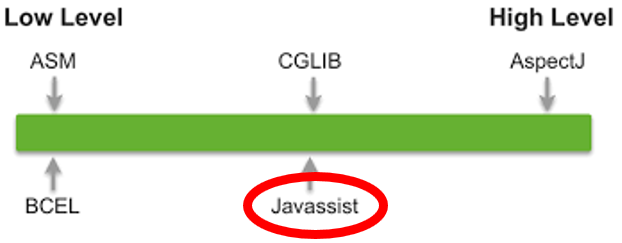
\includegraphics[width=0.8\linewidth]{bytecodeModificationLevels}
\caption{Bytecode modification levels}
  \label{fig:bytecodeModificationLevels}
\end{figure}

Unlike many other libraries Javassist offers two levels of API: source level and bytecode level (See figure \ref{fig:bytecodeModificationLevels}). Using the source-level API, the user can edit a class file without any familiarity with the specifications of the Java bytecode. Only knowing the Java language is enough because the API is designed only with the vocabulary of Java. On this level the programmer just has to write normal source code and Javassist compiles it automatically. The bytecode level allows the user to modify classes directly in binary form like other editors, e.g. ASM.

At this point, let us look at a small example to give you an idea how the bytecode manipulation works.

\begin{figure}[H]
\centering
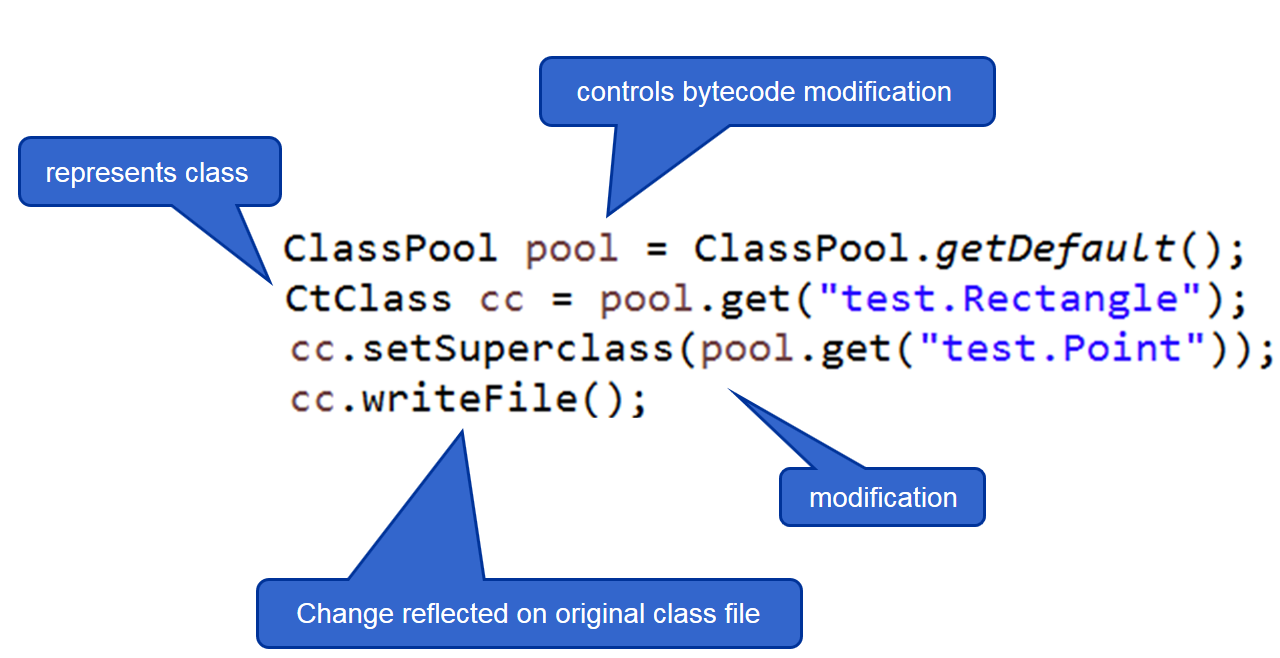
\includegraphics[width=0.8\linewidth]{javassistExample}
\caption{Javassist example}
  \label{fig:javassistExample}
\end{figure}

First a ClassPool object is obtained that controls bytecode modification with Javassist. With the ClassPool a class file can be read on demand for constructing a CtClass object. The class CtClass (compile-time class) is just an abstract representation of a class file which means all manipulations are performed on the CtClass. With the method invocation “get()” on ClassPoola reference to the class file “test.Rectangle” is obtained. In this example the superclass of “test.Rectangle” is just changed to “test.Point”. If the changes are done, the method call “writeFile()” on CtClass is necessary to make sure that the changes are reflected on the original class file.

\begin{figure}[H]
\centering
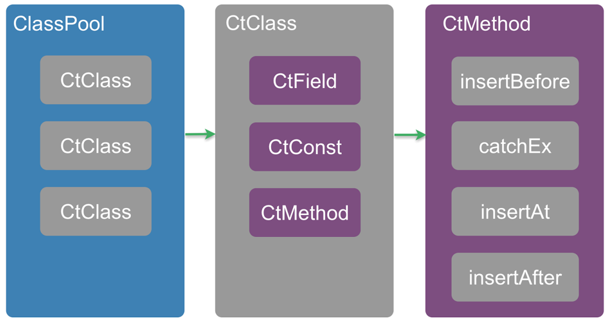
\includegraphics[width=0.8\linewidth]{javassistModules}
\caption{Javassist Modules}
  \label{fig:javassistModules}
\end{figure}

Figure \ref{fig:javassistModules} gives you an understanding/overview how the main part of bytecode manipulation with Javassist is built up. The ClassPool is nothing else than a container of multiple CtClasses. As described before CtClass is just the abstract representation of a class file on which modifications are done. Like typical classes, it can hold several compile-time fields, constants or methods. While speaking about bytecode manipulation all the time, nothing but editing method is manly meant. It is possible to insert source code at the beginning of the method body, at the end or at a specific line. Next to these options a “catchBlock” can even be added.

\begin{figure}[H]
\centering
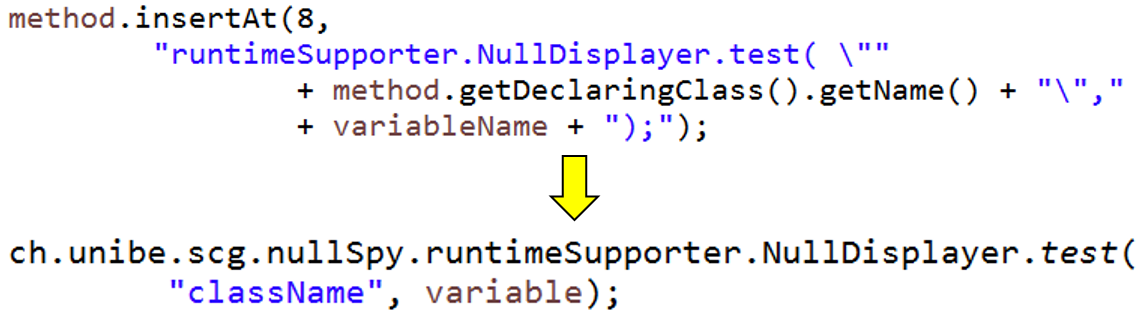
\includegraphics[width=0.9\linewidth]{insertionCodeExample}
\caption{Inserting code example}
  \label{fig:insertionCodeExample}
\end{figure}

\section{JAD}
JAva Decompiler\footnote{\url{https://sourceforge.net/projects/jadclipse/}} is a decompiler and a Eclipe plugin for the programming language Java. A short explanation what a decompiler is: a computer program that takes an executable file as input, and attempts to create a high level, compatible source file that does the same thing. So it is used in software reverse engineering.

JAD is used in NullSpy since after running NullSpy on a project only the modificated bytecodes are available. But to simplify the check if the modification by Javassist, e.g. inserting source code, has succeeded, a decompiler is needed.

\chapter{NullSpy}
In which we understand what the problem is in detail.

\section{High level overview}
blb...

\section{Low level overview}
...

\section{Challanges}
...

\section{Limitations}
...

\chapter{Validation}
In which you show how well the solution works.

\section{JHotDraw}
JHotDraw
To check whether the logic of the bytecode manipulation in this project NullSpy is working as desired, we had to perform them on a large working project. Thanks to Nevena Milojkovic and her experience with the combination Javassist and JHotDraw we as well decided to test NullSpy on the project JHotDraw.
It is an open-source Java GUI framework for technical and structured Graphics. Its original authors have been Erich Gamma and Thomas Eggenschwiler. 

\chapter {Conclusion and Future Work}
In which we step back, have a critical look at the entire work, then conclude, and learn what lays beyond this thesis.

\chapter {Anleitung zu wissenschaftlichen Arbeiten}
This consists of additional documentation, e.g. a tutorial, user guide etc.
Required by the Informatik regulation.

%END Doc
%-------------------------------------------------------

\bibliography{thesis}
\bibliographystyle{plain}

\end{document}